%!TEX root=../document.tex

\section{Ergebnisse}
\label{sec:Ergebnisse}
Es standen ein paar Beispielklassen zur Verfügung, welche von Moodle heruntergeladen wurden. Darin befanden sich zwei Klassen, eine davon beschrieb die den LDAP Connector (wird später noch im Protokoll erwähnt) und die andere erklärte ein paar Code-Snippets zur Verschlüsselung und Encoding. Unter anderem gab es schon zwei Utils-Methoden, welche das Encoding und Umwandeln deutlich erleichtert haben.

\section{Naming Service}
\label{sec:Naming Service}
Im vorherigen Schuljahr gab es eine Aufgabe, bei der es sich um die Umsetzung und Konfiguration eines Naming Service für Java gehandelt hat. Da einigen Schülern diese Aufgabe nicht mehr zur Verfügung steht, wurde eine Virtuelle Maschine bereitgestellt, welche ein voll funktionstüchtiges LDAP besaß.

Wie die Grafik in der Aufgabenstellung beschreibt wird der \textbf{public}-Key vom \textbf{Service} im LDAP-Verzeichnis eingetragen und vom \textbf{Client} ausgelesen.

\begin{lstlisting}[style=Java, caption=LDAP store public-Key in LDAP]
public void storePubKeyinLDAP(){
  LDAPConnector ldapConnector = new LDAPConnector(ldapHost);
  try {
    ldapConnector.updateAttribute("cn=group.Service1,dc=nodomain,dc=com", "description", UsedUtils.toHexString(pubKey.getEncoded()));
    System.out.println("public key stored in LDAP: "+ UsedUtils.toHexString(pubKey.getEncoded()));
    }catch (Exception e){
    e.printStackTrace();
  }
}
\end{lstlisting}

\section{Aufbau, Verschluesselung und Kommunikation}
\label{sec:Aufbau}
Die asymmetrische Verschlüsselung passiert hierbei über den Namensdienst, dem Service und dem Client. Wie schon vorher erwähnt stellt der Service seinen
\textbf{public}-Key in LDAP und der Client holt sich diesen. Er generiert einen \textbf{Secret}-Key für die symmetrische Verschlüsselung im späteren Verlauf.
Der Client wrappt nun seinen \textbf{Secret}-Key mit dem \textbf{public}-Key vom Service und übermittelt diesen über \textbf{Sockets} an den Service. Der Service
decrypted den verschlüsselten Secret-Key mit dem \textbf{private}-Key und mit diesem entschlüsselten \textbf{Secret}-Key wird eine Nachricht verschlüsselt. Diese Nachricht
wird über \textbf{Sockets} zurück an den Client übertragen und von diesem entschlüsselt und ausgegeben.

\section{Code}

Der komplette Source-Code befindet sich in meinem Git-Repository unter dem Link:
\url{https://github.com/mseidl-tgm/5YHITM/tree/master/DEZSYS}

\newpage
\subsection{Service}

Die wichtigste Methode \textit{genKeyPair} generiert ein Schlüsselpaar, welches in \textbf{public}- und \textbf{private}-Key unterteilt werden kann.
Hierfür gibt es einen sogenannten \textit{KeyPairGenerator}. Am Schluß werden noch die Attribute, welche die Keys enthalten sollen, gesetzt.


\begin{lstlisting}[style=Java, caption= RSA KeyPair generation]
    public void genKeyPair(){
	    try {
		    KeyPairGenerator generator = KeyPairGenerator.getInstance("RSA");
		    SecureRandom random = SecureRandom.getInstance("SHA1PRNG", "SUN");
		    generator.initialize(1024, random);
			this.keyPair = generator.generateKeyPair();
    
	    } catch (Exception e) {
		    e.printStackTrace();
	    }
	    pubKey = keyPair.getPublic();
	    privKey = keyPair.getPrivate();
    
    }

\end{lstlisting}

Der folgende Code-Snippet beschreibt die Funktion \textit{encryptMessage}, in welcher die an den Client zu sendende Nachricht verschlüsselt wird.
Es wird ein neuer \textbf{Cipher} generiert, welcher die Encryption übernimmt. Es wird der \textbf{Secret}-Key angegeben, um die Nachricht richtig zu
Verschlüsseln.
\newline

\begin{lstlisting}[style=Java, caption= Message encrypting]
	public byte[] encryptMessage(){
		try {
			Cipher cipher = Cipher.getInstance("AES");
			cipher.init(Cipher.ENCRYPT_MODE, this.secretKey);
			byte[] msgBytes = toSendMessage.getBytes();
			byte[] tmp = cipher.doFinal(msgBytes);
			System.out.println("encrypted Message: "+ UsedUtils.toHexString(tmp));
			return tmp;
		}catch (Exception e){
			e.printStackTrace();
		}
		return null;
	}
\end{lstlisting}

\newpage

\subsection{Client}

Die Methode \textit{encryptSecret} verschlüsselt den generierten Secret-Key mit dem \textbf{public}-Key aus dem LDAP-Verzeichnissystem. Hier wird wieder ein \textbf{Cipher} verwendet um die den Secret-Key zu ''ummanteln''.


\begin{lstlisting}[style=Java, caption= SecretKey encrypting on Client-Side]
    public byte[] encryptSecret(){
	    byte[] tmp;
	    try {
		    Cipher cipher = Cipher.getInstance("RSA");
		    cipher.init(Cipher.WRAP_MODE, this.pubKey);
			tmp = cipher.wrap(secretKey);
		    System.out.println("Secret Key successfully encrypted!" + UsedUtils.toHexString(tmp));
		    return tmp;
		}catch (Exception e){
		    e.printStackTrace();
	    }
	    return null;
    }
\end{lstlisting}

\subsection{UML-Diagramm}
Das Diagramm befindet sich auf der nächsten Seite.

\begin{figure}[!h]
	\begin{center}
		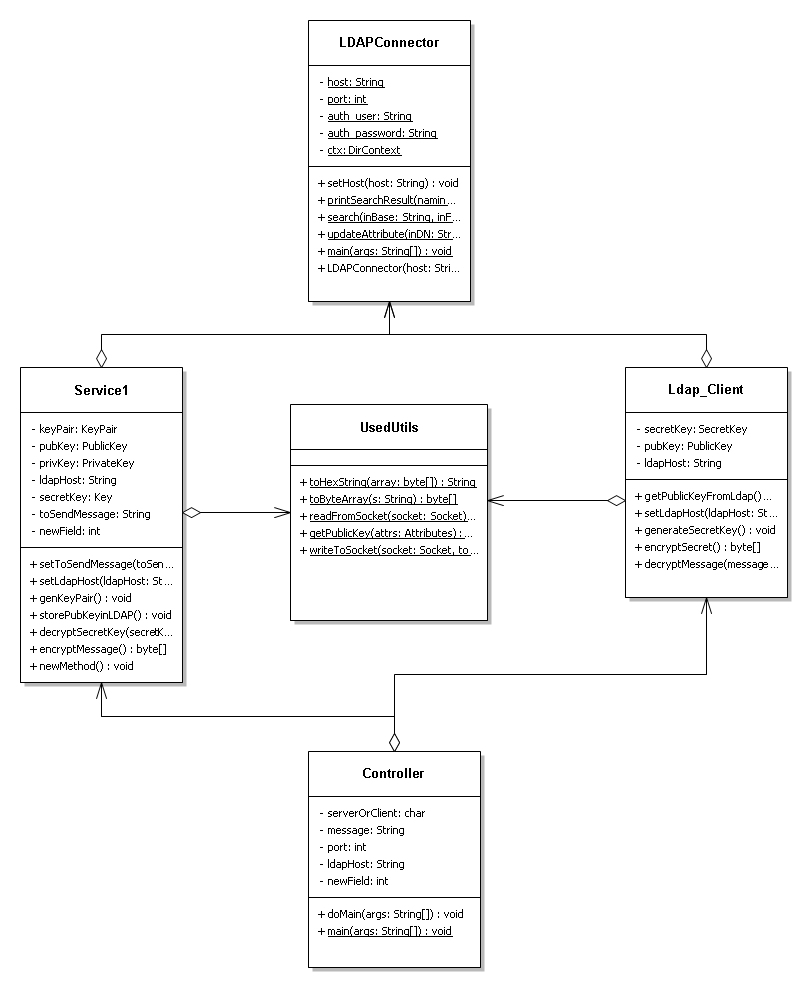
\includegraphics[width=\textwidth]{images/Java_Security_UML}
		\caption{UML-Diagramm des Java-Programms}
		\label{broker}
	\end{center}
\end{figure}

\subsection{Probleme}
Bei den ersten Tests sind einige \textbf{Connection-Probleme} bei den Sockets aufgetreten, welche dann zu \textbf{Null-Pointer-Exceptions} bei der Codierung geführt haben. Diese haben sich aber dann durch Abstraktion der \textbf{readWrite}-Methoden aufgelöst.

\subsection{Zeitaufzeichnung}

\begin{table}[!h]
	\centering
	\caption{Zeitaufzeichnung}
	\label{my-label}
	\begin{tabular}{|l|l|l|}
		\hline
		\multicolumn{1}{|c|}{\textbf{Datum, Anzahl in h}} & \multicolumn{1}{c|}{\textbf{Task}} & \multicolumn{1}{c|}{\textbf{Ort}} \\ \hline
		18.10.2016, 3 h                                   & Diagramentwicklung                 & TGM/daheim                        \\ \hline
		20.10.2016, 4 h                                   & Code-Entwicklung, Debugging        & TGM/daheim                        \\ \hline
		21.10.2016, 2 h                                   & Protkoll, Debugging                & McDonald/daheim                   \\ \hline
	\end{tabular}
\end{table}



